\section{System-level Design}

\subsection{Testbench Architecture}
\subsection{User Interface}

\section{Hardware Design Choices}


\subsection{Randomiser}
With relatively low effort, random testing can provide significant coverage and discover relatively subtle errors~\cite{Duran1}.
LFSRs are a reliable way of generating pseudorandom numbers quickly with low cost~\cite{Hazwani1}.
\subsubsection{LFSR Configurations}

To compare, we can examine an 8-bit LFSR with taps on bit [7,5,4,3].

\textit{Fibonacci} --
Classical option, easier to write and scale in hardware.

\begin{figure}[ht]
  \centering
  \begin{tikzpicture}
  [
    x=1em, y=1em,
    start chain = going right,
    node distance = 0em,
    reg/.style =
      {draw, minimum width=2em, minimum height=2em,outer sep=0pt, on chain},
    every join/.style={-, thick}
  ]
  \node [reg] at (0, 0) (1) {1};
  \node [reg] (2) {};
  \node [reg] (3) {};
  \node [reg] (4) {4};
  \node [reg] (5) {5};
  \node [reg] (6) {6};
  \node [reg] (7) {};
  \node [reg] (8) {8};

  \node[xor gate US,draw,rotate=180] at (2.5, 2) (a) {};
  \node[xor gate US,draw,rotate=180] at (5.5, 3) (b) {};
  \node[xor gate US,draw,rotate=180] at (8.5, 4) (c) {};

  \draw (4.north)  |- (a.input 1);
  \draw (5.north)  |- (b.input 1);
  \draw (6.north)  |- (c.input 1);

  \draw (b.output) to[-|-] (a.input 2);
  \draw (c.output) to[-|-] (b.input 2);
  \draw (8.north)       |- (c.input 2);

  \draw (a.output) -- (-2, 2) |- (1.west);

\end{tikzpicture}
  \caption{Fibonacci Configuration}
  \label{FibLFSR}
\end{figure}

\textit{Galois} --
Harder to write if variable length is desired, but faster in hardware.

\begin{figure}[ht]
  \centering
  \begin{tikzpicture}
  [
    x=1em, y=1em,
    start chain = going right,
    node distance = 0em,
    reg/.style =
      {draw, minimum width=2em, minimum height=2em, outer sep=0pt, on chain},
    spa/.style =
      {minimum width=3em, minimum height=2em, outer sep=0pt, on chain},
    every join/.style={-, thick}
  ]
  \node [reg] at (0, 0) (1) {1};
  \node [reg] (2) {};
  \node [reg] (3) {};
  \node [reg] (4) {4};
  \node [spa] ()  {};
  \node [reg] (5) {5};
  \node [spa] ()  {};
  \node [reg] (6) {6};
  \node [spa] ()  {};
  \node [reg] (7) {};
  \node [reg] (8) {8};

  \node[xor gate US,draw,rotate=180] at  (8.5, 0) (a) {};
  \node[xor gate US,draw,rotate=180] at (13.5, 0) (b) {};
  \node[xor gate US,draw,rotate=180] at (18.5, 0) (c) {};

  \draw (1.west) -| (-2, -2) -- (25,-2) |- (8.east);

  \draw  (9.7,-2) |- (a.input 1);
  \draw (14.7,-2) |- (b.input 1);
  \draw (19.7,-2) |- (c.input 1);

  \draw (a.input 2-|5.west) -- (a.input 2);
  \draw (b.input 2-|6.west) -- (b.input 2);
  \draw (c.input 2-|7.west) -- (c.input 2);

  \draw (a.output) -- (4.east);
  \draw (b.output) -- (5.east);
  \draw (c.output) -- (6.east);

\end{tikzpicture}
  \caption{Galois Configuration}
  \label{GalLFSR}
\end{figure}

\textit{Others} --
Other LFSR configurations such as Xorshift~\cite{Marsaglia1} exists, but they are much slower in hardware.

\subsubsection{Randomiser Structure}

\textit{Horizontal} --
Easy to build, easy to test with.

\begin{figure}[ht]
  \centering
  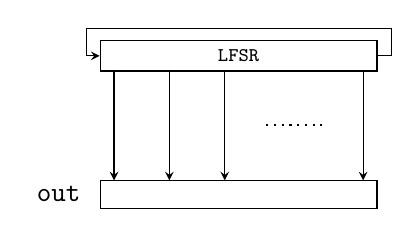
\begin{tikzpicture}
  [
    x=1em, y=1em
  ]
  \node at (-1.5, 0) {\texttt{out}};
  \node [draw,minimum height=1em, minimum width=10em] at (5, 0) (o) {};
  \node [draw,minimum height=1em, minimum width=10em] at (5, 5) (1) {\scriptsize \texttt{LFSR}};
  \draw [->, >=stealth] (1.east) -| ++(0.5, 1) -- ++(-11, 0) |- (1.west);
  \foreach \pos [count=\idx] in {0.5, 2.5, 4.5, 9.5}{
    \draw [->, >=stealth] (\pos, 4.5) -- (\pos, 0.5);
  }
  \draw [dotted, thick] (6, 2.5) -- (8, 2.5);

\end{tikzpicture}
  \caption{Horizontal Structure}
  \label{HoriLFSR}
\end{figure}

\textit{Vertical} --
Nice randomness, more scalable, need to seed all the LFSRs differently.

\begin{figure}[ht]
  \centering
  \begin{tikzpicture}
  [
    x=1em, y=1em
  ]
  \node at (-1.5, 0) {\texttt{out}};
  \node [draw,minimum height=1em, minimum width=10em] at (5, 0) (o) {};
  \foreach \pos [count=\idx] in {0.5, 2.5, 4.5, 9.5}{
    \node [draw,minimum height=1em, minimum width=5em, rotate around={90:(0, 0)}] at (\pos, 5) (\idx) {\scriptsize \texttt{LFSR}};
    \draw [->, >=stealth] (\idx.west) -- (\idx.west|-o.north);
    \draw [->, >=stealth] ($(\idx.west)-(0, 0.5)$) -| (\pos-1,8) -| (\idx.east);
  }

  \draw [dotted, thick] (6, 5) -- (7.5, 5);

\end{tikzpicture}
  \caption{Vertical Structure}
  \label{VertLFSR}
\end{figure}

\subsection{Driver}
\subsubsection{Dual Driver System}
One driver focusses on fast stress tests,
The other allows handwritten tests to coexist with random tests.
They can be switched in software.

\subsection{Monitor}


\subsection{Scoreboard}

\section{Software Design Choices}

\subsection{Code Structure}
